
%====================================================================
\chapter{Operations Within the Enclave}
\label{sec:Enclave}
%====================================================================

A number of interactions with TIS may occur within the
Enclave.
These interactions leave some of the $IDStation$ state unchanged.

\begin{schema}{EnclaveContextC}
        \Delta IDStationC
\\      RealWorldChangesC
\also
        \Xi TISControlledRealWorldC
\also
        \Xi UserTokenC
\\      \Xi FingerC
\\      \Xi StatsC
\\      \Xi CertificateStore
\\      \Xi Keyboard
\where
        fingerTimeout' = fingerTimeout
\\      tokenRemovalTimeoutC' = tokenRemovalTimeoutC
\end{schema}
\begin{Zcomment}
\item
The following state components may change $KeyStoreC$, 
$FloppyC$, $ConfigC$, $AdminC$, $InternalC$, $AdminTokenC$
$DoorLatchAlarmC$ and $AuditLogC$. 
\item
The components of the real world controlled by TIS remain unchanged.
\end{Zcomment}

The operations that may occur within the enclave include
administrator operations and the ID station enrolment. These are
described in this section.

%-------------------------------------------------------------------------
\section{Enrolment of an ID Station}
%-------------------------------------------------------------------------

\begin{traceunit}{FD.Enclave.TISEnrolOp}
\traceto{FS.Enclave.TISEnrolOp}
\end{traceunit}

Before TIS can be used it must be enrolled.

We assume
that the initial enrolment is the only possible enrolment activity.

Enrolment is a multi-phase activity, the state transistions for an
enrolment are given in Figure \ref{fig:enrol}. Before enrolment the
system is in state $notEnrolled$ and, on successful completion, it
enters the $quiescent$ state.

\begin{figure}[htbp]
  \begin{center}
    \leavevmode
    \resizebox{\textwidth}{!}{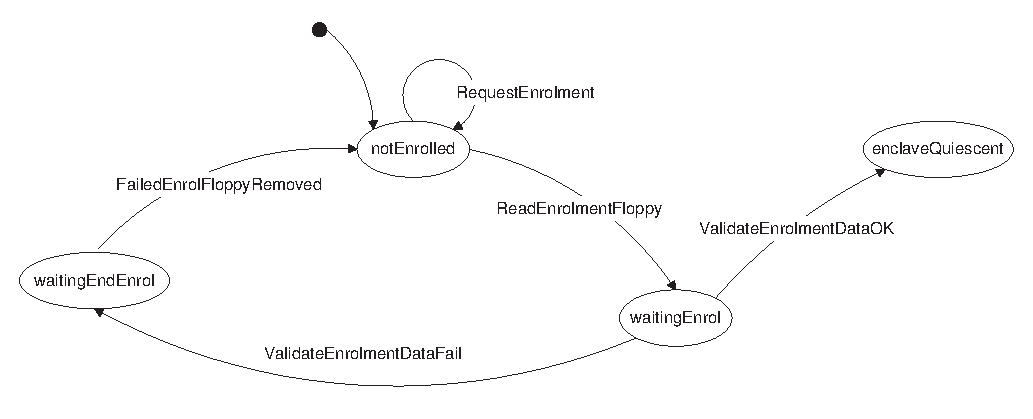
\includegraphics{50_1_enrol.eps}}
    \caption{Enrolment state transitions}
    \label{fig:enrol}
  \end{center}
\end{figure}

The context for all enrolment operations is given below.

\begin{schema}{EnrolContextC}
        EnclaveContextC
\also
        \Xi AdminC
\\      \Xi AdminTokenC
\\      \Xi DoorLatchAlarmC
\\      \Xi ConfigC
\\      \Xi FloppyC
\\      AddElementsToLogC
\\      LogChangeC
\where
        auditTypes~ newElements? \subseteq ENROL\_ELEMENTS \cup USER\_INDEPENDENT\_ELEMENTS
\end{schema}

\begin{Zcomment}
\item
The following state components may change 
$KeyStore$, $Internal$ and  $AuditLog$. 
\end{Zcomment}


%...................................
\subsection{Requesting Enrolment}
%...................................


\begin{traceunit}{FD.Enclave.RequestEnrolment}
\traceto{FS.Enclave.RequestEnrolment}
\end{traceunit}


The ID station will request enrolment while there is no Floppy
present. This will occur until a successful enrolment is achieved.

\begin{schema}{RequestEnrolmentC}
        EnrolContextC
\also
        \Xi KeyStoreC
\\      \Xi FloppyC
\where
        enclaveStatusC = notEnrolled
\\      floppyPresenceC = absent
\also
        currentScreenC'.screenMsgC = insertEnrolmentDataC
\also
        enclaveStatusC' = enclaveStatusC
\\      statusC' = statusC
\\      currentDisplayC' = blank
\also
        auditTypes~ newElements? \cap ENROL\_ELEMENTS = \emptyset
\end{schema}


\begin{traceunit}{FD.Enclave.ReadEnrolmentFloppy}
\traceto{FS.Enclave.ReadEnrolmentFloppy}
\end{traceunit}

If a floppy is present then TIS goes on to validate the
contents. Nothing is written to the log at this stage as log entries
will be made on successful or failed enrolment.

\begin{schema}{ReadEnrolmentFloppyC}
        EnrolContextC
\also
        ReadFloppyC
\\      \Xi KeyStoreC
\where
        enclaveStatusC = notEnrolled
\\      floppyPresenceC = present
\also
        currentScreenC'.screenMsgC = validatingEnrolmentDataC 
\also
        enclaveStatusC' = waitingEnrol     
\\      statusC' = statusC
\\      currentDisplayC' = blank                         
\also
        auditTypes~ newElements? \cap ENROL\_ELEMENTS = \emptyset
\end{schema}

\begin{zed}
        ReadEnrolmentDataC \defs (ReadEnrolmentFloppyC \lor
        RequestEnrolmentC) \hide (newElements? )
\end{zed}

%.........................................
\subsection{Validating Enrolment data from Floppy}
%.........................................

For the enrolment data to be acceptable the data on the floppy must be
valid enrolment data with the ID Station certificate containing this
ID station's public key. 

\begin{schema}{EnrolmentDataOKC}
        FloppyC
\\      KeyStoreC
\where
        currentFloppyC \in \ran enrolmentFileC
\\      (\exists ValidEnrolC @ \theta ValidEnrolC = enrolmentFileC \inv
currentFloppyC)
\end{schema}

\begin{traceunit}{FD.Enclave.ValidateEnrolmentDataOK}
\traceto{FS.Enclave.ValidateEnrolmentDataOK}
\end{traceunit}

If the data on the floppy is acceptable to be used for enrolment then
the Key store is updated. From this point the system is available for
use both by users entering the enclave and by administrators.

A successful enrolment is recorded in the audit log, no user can be
associated with the enrolment activity.

\begin{schema}{ValidateEnrolmentDataOKC}
        EnrolContextC
\also
        \Xi FloppyC
\\      UpdateKeyStoreFromFloppyC
\where
        enclaveStatusC = waitingEnrol
\also
        EnrolmentDataOKC
\also
        currentScreenC'.screenMsgC = welcomeAdminC
\also
        enclaveStatusC' = enclaveQuiescent 
\\      statusC' = quiescent
\\      currentDisplayC' = welcome
\also
        auditTypes~ newElements? \cap ENROL\_ELEMENTS = 
        \{ enrolmentCompleteElement \} 
\also
        \exists_1 element : AuditC @ element \in newElements? 
\\ \t1  \land element.elementId = enrolmentCompleteElement
\\ \t1  \land element.logTime \in nowC \upto nowC'
\\ \t1  \land element.user = noUser
\\ \t1  \land element.severity = information
\\ \t1  \land element.description = noDescription
\end{schema}

\begin{traceunit}{FD.Enclave.ValidateEnrolmentDataFail}
\traceto{FS.Enclave.ValidateEnrolmentDataFail}
\end{traceunit}

If the enrolment fails then TIS waits for the floppy to be removed
before prompting for new enrolment data. 

\begin{schema}{ValidateEnrolmentDataFailC}
        EnrolContextC
\also
        \Xi KeyStoreC
\\      \Xi FloppyC
\where
        enclaveStatusC = waitingEnrol
\also
        \lnot EnrolmentDataOKC
\also
        currentScreenC'.screenMsgC = enrolmentFailedC
\also
        enclaveStatusC' = waitingEndEnrol
\\      statusC' = statusC
\\      currentDisplayC' = blank
\also
        auditTypes~ newElements? \cap ENROL\_ELEMENTS = 
        \{ enrolmentFailedElement \} 
\also
        \exists_1 element : AuditC @ element \in newElements? 
\\ \t1  \land element.elementId = enrolmentFailedElement
\\ \t1  \land element.logTime \in nowC \upto nowC'
\\ \t1  \land element.user = noUser
\\ \t1  \land element.severity = warning
\end{schema}
\begin{Zcomment}
\item
The value of the $description$ is left free here as the description component of the audit element may contain
information relating to the reason that the enrolment data failed.
This is not formally stated.
\end{Zcomment}

\begin{zed}
        ValidateEnrolmentDataC \defs ValidateEnrolmentDataOKC \lor
          ValidateEnrolmentDataFailC
\end{zed}

%.........................................
\subsection{Completing a failed Enrolment}
%.........................................

A failed enrolment will only terminate once the floppy has been
removed, otherwise the system would repeatedly try to validate the
same floppy.

\begin{traceunit}{FD.Enclave.FailedEnrolFloppyRemoved}
\traceto{FS.Enclave.FailedEnrolFloppyRemoved}
\end{traceunit}


Once the floppy has been removed the administrator is prompted for
enrolment data again. We do not log the removal of the floppy in the
audit log.

\begin{schema}{FailedEnrolFloppyRemovedC}
        EnrolContextC
\also
        \Xi FloppyC
\\      \Xi KeyStoreC
\where
        enclaveStatusC = waitingEndEnrol
\\      floppyPresenceC = absent
\also
        currentScreenC'.screenMsgC = insertEnrolmentDataC
\also
        enclaveStatusC' = notEnrolled
\\      statusC' = statusC
\\      currentDisplayC' = blank
\also
        auditTypes~ newElements? \cap ENROL\_ELEMENTS = \emptyset
\end{schema}

\begin{traceunit}{FD.Enclave.WaitingFloppyRemoval}
\traceto{FS.Enclave.WaitingFloppyRemoval}
\end{traceunit}

\begin{schema}{WaitingFloppyRemovalC}
        EnclaveContextC
\also
        \Xi IDStationC
\where
        enclaveStatusC = waitingEndEnrol
\\      floppyPresenceC = present
\end{schema}

\begin{zed}
        CompleteFailedEnrolmentC \defs FailedEnrolFloppyRemovedC 
         \lor WaitingFloppyRemovalC
\end{zed}

%..........................................
\subsection{The Complete Enrolment}
%..........................................

The complete enrolment process involves reading the enrolment data,
validating it and, in the case of a failure waiting for the system to
be in a state where it can try another enrolment.

\begin{zed}
        TISEnrolOpC \defs (ReadEnrolmentDataC \lor
ValidateEnrolmentDataC 
\\      \t4 \lor CompleteFailedEnrolmentC) \hide (newElements?)
\end{zed}

%-----------------------------------------------------------------------
\section{Administrator Token Tear}
%-----------------------------------------------------------------------

The action of removing the administrator Token will result in the
administrator being logged out of the system.

This may happen at any point once a token has been inserted into the
reader. As soon as the adminitrator's token is torn this action will
be logged. 


\begin{schema}{AdminTokenTearC}
         EnclaveContextC
\\       AddElementsToLogC
\\       LogChangeC
\also
        ClearAdminToken
\\      \Xi ConfigC
\\      \Xi FloppyC
\\      ResetScreenMessageC
\where
        adminTokenPresenceC = absent
\also   
        currentScreenC'.screenMsgC = welcomeAdminC 
\\      statusC' = statusC
\\      currentDisplayC' = currentDisplayC
\also
        enclaveStatusC' = enclaveQuiescent
\end{schema}
If the admin token is torn while the system is processing an activity
within the enclave then the activity will be stopped.

\begin{schema}{BadAdminTokenTearC} 
        AdminTokenTearC
\where
        AdminHasDeparted
\\      enclaveStatusC \in \{ gotAdminToken, waitingStartAdminOp,
        waitingFinishAdminOp \} 
\also
        auditTypes~ newElements? \cap ADMIN\_ELEMENTS = 
        \{ adminTokenRemovedElement \} 
\also
        \exists_1 element : AuditC @ element \in newElements? 
\\ \t1  \land element.elementId = adminTokenRemovedElement
\\ \t1  \land element.logTime \in nowC \upto nowC'
\\ \t1  \land element.user = extractUser~ currentAdminTokenC
\\ \t1  \land element.severity = warning
\\ \t1  \land element.description = noDescription
\end{schema}


\begin{traceunit}{FD.Enclave.LoginAborted}
\traceto{FS.Enclave.LoginAborted}
\end{traceunit}

If the token is torn during the log on validation process then there
is no need to log off the administrator.

\begin{schema}{LoginAbortedC}
        BadAdminTokenTearC
\\      \Xi AdminC
\where
        enclaveStatusC = gotAdminToken
\end{schema}



%----------------------------------------------------------------------
\section{Administrator Login}
%----------------------------------------------------------------------


An Administrator logs into TIS by inserting a valid token
into the $adminToken$ reader. The authorisation certificate is
verified and the user is logged in with the privileges indicated on
the card.

Once the administrator is successfully logged into TIS, the system
records that there is a role present. The process of logging on is
given by the state transition diagram in Figure \ref{fig:logon}

\begin{figure}[htbp]
  \begin{center}
    \leavevmode
    \resizebox{\textwidth}{!}{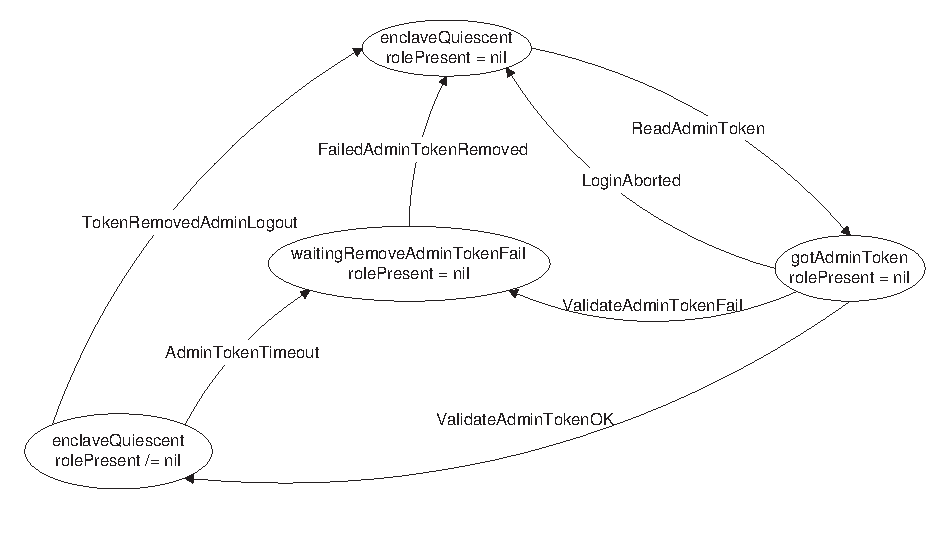
\includegraphics{50_1_admin.eps}}
    \caption{Administrator logon state transitions}
    \label{fig:logon}
  \end{center}
\end{figure}

The context for administrator login is given below.

\begin{schema}{LoginContextC}
        EnclaveContextC
\also
        \Xi KeyStoreC
\\      \Xi DoorLatchAlarmC
\\      \Xi ConfigC
\\      AddElementsToLogC
\\      LogChangeC
\where
        statusC' = statusC
\\      currentDisplayC' = currentDisplayC
\end{schema}

\begin{Zcomment}
\item
The following state components may change 
$AdminC$, $InternalC$ and  $AuditLogC$. 
\end{Zcomment}

%..........................................
\subsection{Read Administrator Token}
%..........................................

\begin{traceunit}{FD.Enclave.GetPresentAdminToken}
\traceto{FS.Enclave.ReadAdminToken}
\end{traceunit}

When the admin token is read the action is audited and the internal
status changes. No other aspects of the system are modified.

An administrator can only log on when there is no user entry activity
in progress or TIS is waiting for a failed user token to be removed
from the token reader outside of the enclave.

\begin{schema}{GetPresentAdminTokenC}
         LoginContextC
\also
        \Xi AdminC
\\      ReadAdminTokenC
\where
        AdminLogonCanStart
\also
	enclaveStatusC' = gotAdminToken
\also
        currentScreenC' = currentScreenC
\also
        auditTypes~ newElements? \cap ADMIN\_ELEMENTS = 
        \{ adminTokenPresentElement \} 
\also
        \exists_1 element : AuditC @ element \in newElements? 
\\ \t1  \land element.elementId = adminTokenPresentElement
\\ \t1  \land element.logTime \in nowC \upto nowC'
\\ \t1  \land element.user = extractUser~ currentAdminTokenC'
\\ \t1  \land element.severity = information
\\ \t1  \land element.description = noDescription
\end{schema}

The operation to read the token is as follows:

\begin{zed}
        TISReadAdminTokenC \defs 
                GetPresentAdminTokenC \hide (newElements?)   
\end{zed}

%..........................................
\subsection{Validate Administrator Token}
%..........................................

An administrator's token is considered valid if it contains a valid
and current 
authorisation certificate. Additionally the
privileges assigned to the user within the authorisation certificate
must indicate that the user is actually an administrator.

\begin{traceunit}{FD.Enclave.ValidateAdminTokenOK}
\traceto{FS.Enclave.ValidateAdminTokenOK}
\end{traceunit}


If the token can be validated then the administrator is logged onto
TIS.

\begin{schema}{ValidateAdminTokenOKC}
        LoginContextC
\also
        \Xi AdminTokenC
\where
        \lnot AdminHasDeparted
\\      enclaveStatusC = gotAdminToken
\also
        AdminTokenOKC
\also   
        currentScreenC'.screenMsgC = requestAdminOpC 
\also
        enclaveStatusC' = enclaveQuiescent
\also
        \exists requiredRole? : ADMINPRIVILEGE @ AdminLogonC 
\\ \t1  \land requiredRole? = (extractAuthCert~ (\The (goodTC \inv
currentAdminTokenC). authCertC)).roleC 
\also
        auditTypes~ newElements? \cap ADMIN\_ELEMENTS = 
        \{ adminTokenValidElement \} 
\also
        \exists_1 element : AuditC @ element \in newElements? 
\\ \t1  \land element.elementId = adminTokenValidElement
\\ \t1  \land element.logTime \in nowC \upto nowC'
\\ \t1  \land element.user = extractUser~ currentAdminTokenC'
\\ \t1  \land element.severity = information
\\ \t1  \land element.description = noDescription
\end{schema}

\begin{traceunit}{FD.Enclave.ValidateAdminTokenFail}
\traceto{FS.Enclave.ValidateAdminTokenFail}
\end{traceunit}

If the token can not be validated then TIS waits for it to be removed.

\begin{schema}{ValidateAdminTokenFailC}
        LoginContextC
\also
        \Xi AdminTokenC
\\      \Xi AdminC
\where
        \lnot AdminHasDeparted
\\      enclaveStatusC = gotAdminToken
\also
        \lnot AdminTokenOKC
\also
        currentScreenC'.screenMsgC = removeAdminTokenC
\also
        enclaveStatusC' = waitingRemoveAdminTokenFail
\also
        auditTypes~ newElements? \cap ADMIN\_ELEMENTS = 
        \{ adminTokenInvalidElement \} 
\also
        \exists_1 element : AuditC; description! : TEXT @ 
\\ \t1  element \in newElements? 
\\ \t1  \land element.elementId = adminTokenInvalidElement
\\ \t1  \land element.logTime \in nowC \upto nowC'
\\ \t1  \land element.user = extractUser~ currentAdminTokenC'
\\ \t1  \land element.severity = warning
\\ \t1  \land element.description = description! \land AdminTokenNotOK
\end{schema}
\begin{Zcomment}
\item
$AdminTokenNotOK$ defines the value of the descriptive text applicable
based on the reason for the unacceptability of the token.
\end{Zcomment}


\begin{zed}
        TISValidateAdminTokenC \defs (ValidateAdminTokenOKC \lor
        ValidateAdminTokenFailC 
\\ \t4  \lor
        LoginAbortedC )
        \hide (newElements?)
\end{zed}

\subsection{Complete Failed Administrator Logon}

If an administrator token has failed to be accepted by TIS 
then no further actions can take place in the enclave until it has 
been removed.

\begin{traceunit}{FD.Enclave.FailedAdminTokenRemoved}
\traceto{FS.Enclave.FailedAdminTokenRemoved}
\end{traceunit}


The administrator token may be removed at any point during a user
entry, hence the context for this
activity does not place restrictions on the value of $status$.

When the admin token is removed TIS returns to a state ready
to accept another administrator logon.

\begin{schema}{FailedAdminTokenRemovedC}
        LoginContextC
\also
        \Xi AdminC
\\      ClearAdminToken
\where
        AdminHasDeparted
\\      enclaveStatusC = waitingRemoveAdminTokenFail
\also
        currentScreenC'.screenMsgC = welcomeAdminC
\also
        enclaveStatusC' = enclaveQuiescent
\also
        statusC' = statusC
\\      currentDisplayC' = currentDisplayC
\also
        auditTypes~ newElements? \cap ADMIN\_ELEMENTS = 
        \{ adminTokenRemovedElement \} 
\also
        \exists_1 element : AuditC @ element \in newElements? 
\\ \t1  \land element.elementId = adminTokenRemovedElement
\\ \t1  \land element.logTime \in nowC \upto nowC'
\\ \t1  \land element.user = extractUser~ currentAdminTokenC
\\ \t1  \land element.severity = information
\\ \t1  \land element.description = noDescription
\end{schema}

The case where the token is not removed will be captured within the
model of the system being idle.

\begin{zed}
        TISCompleteFailedAdminLogonC \defs FailedAdminTokenRemovedC 

\end{zed}

%...............................................
\subsection{The Complete Administrator Logon}
%...............................................

\begin{traceunit}{FD.Enclave.TISAdminLogin}
\traceto{FS.Enclave.TISAdminLogin}
\end{traceunit}

The complete administrator logon process, from the point that the
system has detected the presence of a token in the administrator
reader, involves 
validating the administrator token and, in the case of a failure 
waiting for the system to be in a state where it can try another logon.

\begin{zed}
        TISAdminLogonC \defs TISReadAdminTokenC \lor
        TISValidateAdminTokenC \lor TISCompleteFailedAdminLogonC 
\end{zed}

This can be divided into starting the administrator logon:
\begin{zed}
        TISStartAdminLogonC \defs TISReadAdminTokenC  
\end{zed}
 
and progressing the logon to completion. 
\begin{zed}
        TISProgressAdminLogon \defs 
        TISValidateAdminTokenC \lor TISCompleteFailedAdminLogonC 
\end{zed}

%-----------------------------------------------------------------
\section{Administrator Logout}
\label{sec:AdminLogout}
%-----------------------------------------------------------------

Administrator logout can be achieved in two ways, either the
administrator removes their token from TIS, or the Authorisation
certificate on the token expires, causing the system to automatically
log off the administrator.

\begin{traceunit}{FD.Enclave.AdminLogout}
\traceto{FS.Enclave.AdminLogout}
\end{traceunit}

If TIS is not performing an administrator operation then the
token may be removed to log out the administrator.

\begin{schema}{TokenRemovedAdminLogoutC}
        AdminTokenTearC
\\      AdminLogoutC
\also
        ClearAdminToken
\where        
        PresentAdminHasDeparted
\\      enclaveStatusC = enclaveQuiescent
\also
        auditTypes~ newElements? \cap ADMIN\_ELEMENTS = 
        \{ adminTokenRemovedElement \} 
\also
        \exists_1 element : AuditC @ element \in newElements? 
\\ \t1  \land element.elementId = adminTokenRemovedElement
\\ \t1  \land element.logTime \in nowC \upto nowC'
\\ \t1  \land element.user = extractUser~ currentAdminTokenC
\\ \t1  \land element.severity = information
\\ \t1  \land element.description = noDescription
\end{schema}


\begin{traceunit}{FD.Enclave.BadAdminLogout}
\traceto{FS.Enclave.BadAdminLogout}
\end{traceunit}

If the administrator is performing an operation (other than shutdown) when the token is torn
then the administrator will be logged off.

\begin{schema}{BadAdminLogoutC}
        BadAdminTokenTearC
\\      AdminLogoutC
\where
        PresentAdminHasDeparted
\\      enclaveStatusC \in \{ waitingStartAdminOp, waitingFinishAdminOp
        \}
\end{schema}

\begin{traceunit}{FD.Enclave.AdminTokenTimeout}
\traceto{FS.Enclave.AdminTokenTimeout}
\end{traceunit}


The TIS will automatically logout an administrator whose token
expires. This occurs if the validity period on the Authorisation
certificate expires.

\begin{schema}{AdminTokenTimeoutC}
        LoginContextC
\also
        AdminLogoutC
\\      AddElementsToLogC
\\      ResetScreenMessageC
\where
        AdminTokenHasExpired
\also
        enclaveStatusC' = waitingRemoveAdminTokenFail
\also
        auditTypes~ newElements? \cap ADMIN\_ELEMENTS = 
        \{ adminTokenExpiredElement \} 
\also
        \exists_1 element : AuditC @ element \in newElements? 
\\ \t1  \land element.elementId = adminTokenExpiredElement
\\ \t1  \land element.logTime \in nowC \upto nowC'
\\ \t1  \land element.user = extractUser~ currentAdminTokenC
\\ \t1  \land element.severity = warning
\\ \t1  \land element.description = noDescription
\end{schema}

\begin{traceunit}{FD.Enclave.TISCompleteTimeoutAdminLogout}
\traceto{FS.Enclave.TISCompleteTimeoutAdminLogout}
\end{traceunit}

If the administrator's token expires then it must be removed before
further activities can take place at the TIS console. The behaviour
and conditions are identical to the behaviour when the system waits for a the
administrator to remove their token following a failed logon.

\begin{zed}
TISCompleteTimeoutAdminLogoutC \defs TISCompleteFailedAdminLogonC
\end{zed}

%...........................
\subsection{Complete Administrator Logout}
%............................

\begin{traceunit}{FD.Enclave.TISAdminLogout}
\traceto{FS.Enclave.TISAdminLogout}
\end{traceunit}

The complete administrator logout process which must be performed as
soon as an Administrator needs to be logged out is given below.

\begin{zed}
        TISAdminLogoutC \defs ( TokenRemovedAdminLogoutC \lor
        AdminTokenTimeoutC  
\\ \t4  \lor  BadAdminLogoutC ) \hide (newElements?)
\end{zed}



%-----------------------------------------------------------------
\section{Administrator Operations}
%-----------------------------------------------------------------
An administrator operation can take place as long as an administrator
is present. The operation is started by receiving a valid request to
perform an operation from the keyboard. TIS will ensure that the
requested operation is one compatible with the current role present.

Once the operation is started the behaviour depends on the type of
operation. Operations are either short, and can be implemented in one
phase or they are multi-phase operations. 

$shutdown$ and $overrideLock$ are short operations, while $archiveLog$
and $updateCofigData$ are multi phase operations.

The state transition diagram for administrator operations is given in
Figure \ref{fig:adminOp}

\begin{figure}[htbp]
  \begin{center}
    \leavevmode
    \resizebox{\textwidth}{!}{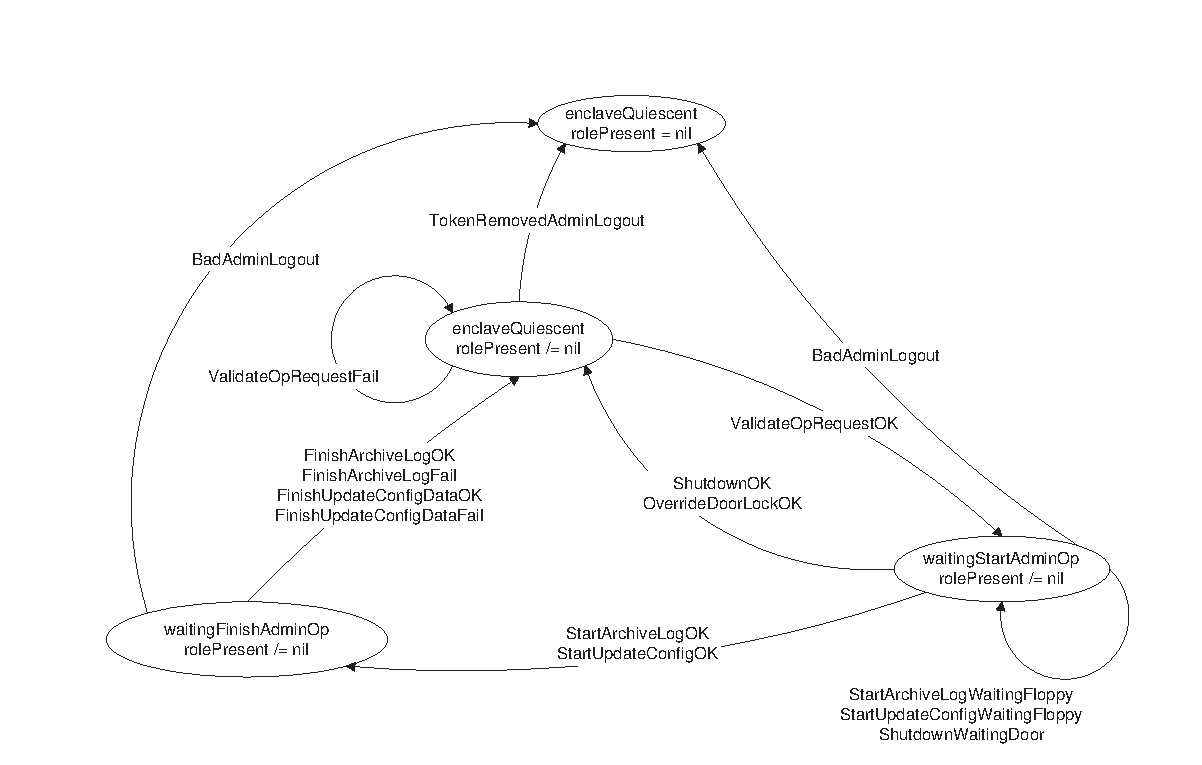
\includegraphics{50_1_adminOp.eps}}
    \caption{Administrator operation state transitions}
    \label{fig:adminOp}
  \end{center}
\end{figure}

All administrator operations have a common context, in which the
$AdminToken$ does not change.
An administrator can only perform an operation when there is no user 
entry activity
in progress or TIS is waiting for a failed user token to be removed
from the token reader outside of the enclave.


\begin{schema}{AdminOpContextC}
        EnclaveContextC
\also
        \Xi KeyStoreC
\\      \Xi AdminTokenC
\\      AddElementsToLogC
\\      LogChangeC
\end{schema}
\begin{Zcomment}
\item
The following state components may change   
$FloppyC$, $ConfigC$, $AdminC$, $DoorLatchAlarmC$ and $AuditLogC$. 
\end{Zcomment}

Once an operation has been started its context is given by:

\begin{schema}{AdminOpStartedContextC}
        AdminOpContextC
\where
        \lnot AdminHasDeparted
\\      enclaveStatusC = waitingStartAdminOp
\also
        statusC' = statusC
\end{schema}

Some operations are multi-phase, the context for completing a
multi-phase operation is given by: 

\begin{schema}{AdminOpFinishContextC}
        AdminOpContextC
\also
        AdminFinishOpC
\where
        \lnot AdminHasDeparted
\\      enclaveStatusC = waitingFinishAdminOp
\also
        statusC' = statusC
\\      currentDisplayC' = currentDisplayC
\also
        enclaveStatusC' = enclaveQuiescent
\end{schema}


%-----------------------------------------------------------------
\section{Starting Operations}
%-----------------------------------------------------------------


All administrator operations are initiated in the same way. This
involves validating the latest keyboard input and determining whether
it is a valid operation request.

TIS only attempts to start an operation if there is an administrator
present and there is no current activity in the enclave.
An administrator can only start an operation when there is no user
entry activity in progress or TIS is waiting for a failed user token 
to be removed from the token reader outside of the enclave.

\begin{schema}{StartOpContextC}
        EnclaveContextC
\also
        \Xi DoorLatchAlarmC
\\      \Xi ConfigC
\\      \Xi FloppyC
\\      \Xi KeyStoreC
\\      \Xi AdminTokenC
\\      AddElementsToLogC
\\      LogChangeC
\where
        AdminOpCanStart        
\also
        statusC' = statusC
\\      currentDisplayC' = currentDisplayC
\end{schema}
\begin{Zcomment}
\item
The following state components may change  
$InternalC$, $AdminC$ and $AuditLogC$. 
\item
We strengthen the precondition of this context to give priority to
starting a
user entry over starting an administrator operation.
\end{Zcomment}

%..........................................
\subsection{Validating an Operation Request}
%..........................................

\begin{traceunit}{FD.Enclave.ValidateOpRequestOK}
\traceto{FS.Enclave.ValidateOpRequestOK}
\end{traceunit}

Once the data from the keyboard has been read this must be validated
to ensure it corresponds to a valid operation.

\begin{axdef}
        keyedDataText : KEYBOARD \fun TEXT
\end{axdef}

\begin{schema}{ValidateOpRequestOKC}
        StartOpContextC
\where
        keyedDataPresenceC = present
\\      \exists request? : KEYBOARD @ request? = keyboardC \land
AdminOpIsAvailable 
\also
        currentScreenC'.screenMsgC = doingOpC
\also
        enclaveStatusC' = waitingStartAdminOp
\also
        \exists requestedOp? : ADMINOP @ requestedOp? = keyedOps \inv
        keyboardC 
\\ \t1  \land AdminStartOpC 
\also
        auditTypes~ newElements? \cap ADMIN\_ELEMENTS = 
        \{ operationStartElement \} 
\also
        \exists_1 element : AuditC @ element \in newElements? 
\\ \t1  \land element.elementId = operationStartElement
\\ \t1  \land element.logTime \in nowC \upto nowC'
\\ \t1  \land element.user = extractUser~ currentAdminTokenC
\\ \t1  \land element.severity = information
\\ \t1  \land element.description = keyedDataText~ keyboardC
\end{schema}

\begin{traceunit}{FD.Enclave.ValidateOpRequestFail}
\traceto{FS.Enclave.ValidateOpRequestFail}
\end{traceunit}


If the data from the keyboard doesn't correspond to an operation that
can be performed at present then the operation is not started and the
attempt to start an illegal operation is logged.

\begin{schema}{ValidateOpRequestFailC}
        StartOpContextC
\also
        \Xi AdminC
\where
        keyedDataPresenceC = present
\\      \exists request? : KEYBOARD @ request? = keyboardC \land
\lnot AdminOpIsAvailable 
\also
        currentScreenC'.screenMsgC = invalidRequestC
\also
        enclaveStatusC' = enclaveStatusC
\also
        auditTypes~ newElements? \cap ADMIN\_ELEMENTS = 
        \{ invalidOpRequestElement \} 
\also
        \exists_1 element : AuditC @ element \in newElements? 
\\ \t1  \land element.elementId = invalidOpRequestElement
\\ \t1  \land element.logTime \in nowC \upto nowC'
\\ \t1  \land element.user = extractUser~ currentAdminTokenC
\\ \t1  \land element.severity = warning
\\ \t1  \land element.description = keyedDataText~ keyboardC
\end{schema}

\begin{traceunit}{FD.Enclave.NoOpRequest}
\traceto{FS.Enclave.NoOpRequest}
\end{traceunit}


If there is no data at the keyboard then TIS waits for user interaction.

\begin{schema}{NoOpRequestC}
        StartOpContextC
\also
        \Xi IDStationC
\where
        keyedDataPresenceC = absent
\end{schema}

\begin{zed}
        ValidateOpRequestC \defs ValidateOpRequestOKC \lor
        ValidateOpRequestFailC \lor NoOpRequestC
\end{zed}

\subsection{Complete Operation Start}
\begin{traceunit}{FD.Enclave.TISStartAdminOp}
\traceto{FS.Enclave.TISStartAdminOp}
\end{traceunit}


The process of starting an administrator operation involves exactly the validation of an
operation request.

\begin{zed}
        TISStartAdminOpC \defs ValidateOpRequestC
\end{zed}


%-------------------------------------------------------------------
\section{Archiving the Log}
%-------------------------------------------------------------------


When the log is archived it is copied to floppy and the internally
held log is truncated.

The internally held log can only be truncated if the write to floppy
succeeds.  

To check that the archive succeeded the floppy is read back and the
data compared with that held by the system.

This is a two phase operation, during the first phase the log is
written to floppy, during the second phase the data on the floppy is
validated. 


%............................
\subsection{Writing the archive Log}
%............................

\begin{traceunit}{FD.Enclave.StartArchiveLogOK}
\traceto{FS.Enclave.StartArchiveLogOK}
\end{traceunit}

The first phase of this operation is to write the archive log to
floppy.

\begin{schema}{StartArchiveLogOKC}
        EnclaveContextC
\also
        \Xi AdminTokenC
\\      \Xi KeyboardC
\\      \Xi KeyStoreC
\\      \Xi Config
\\      \Xi Admin
\\      \Xi AdminToken     
\\      LogChangeC
\also
        newElements? : \finset AuditC
 \where
     \lnot AdminHasDeparted
 \\     enclaveStatusC = waitingStartAdminOp
\also
        \The currentAdminOpC = archiveLog
\\      floppyPresenceC = present
\also
        floppyPresenceC' = floppyPresenceC
\\      currentFloppyC' = currentFloppyC
\also
        currentScreenC'.screenMsgC = doingOpC
\also
        statusC' = statusC
\also
        enclaveStatusC' = waitingFinishAdminOp
\\      (\exists archive! : \finset AuditC @ ArchiveLogC \land
writtenFloppyC' = auditFileC~ archive! )
\end{schema}
\begin{Zcomment}
\item
Note this operation makes other altertions to the audit log so cannot use
the $AdminOpStartedContext$.
\end{Zcomment}
We wait indefinitely for a floppy to be present.

\begin{traceunit}{FD.Enclave.StartArchiveLogWaitingFloppy}
\traceto{FS.Enclave.StartArchiveLogWaitingFloppy}
\end{traceunit}

\begin{schema}{StartArchiveLogWaitingFloppyC}
        AdminOpStartedContextC
\also   
        \Xi ConfigC
\\      \Xi AdminC    
\\      \Xi FloppyC
\where
        \The currentAdminOpC = archiveLog
\\      floppyPresenceC = absent
\also
        currentScreenC'.screenMsgC = insertBlankFloppyC
\\      currentDisplayC' = currentDisplayC
\also
        enclaveStatusC' = enclaveStatusC
\end{schema}

\begin{zed}
        StartArchiveLogC \defs ((StartArchiveLogOKC \semi UpdateFloppyC) 
\\ \t4                  \lor StartArchiveLogWaitingFloppyC  ) \hide
                        (newElements? )
\end{zed}


%............................
\subsection{Clearing the archive Log}
%............................

Note this operation makes altertions to the audit log other than the
addition of elements so cannot use
the $AdminOpFinishContext$. We define a specific context for
completing the archive log.

\begin{schema}{FinishArchiveLogContext}
        EnclaveContextC
\also
        \Xi AdminTokenC
\\      \Xi KeyboardC
\\      \Xi KeyStoreC
\\      \Xi ConfigC
\\      AdminFinishOpC     
\\      \Xi DoorLatchAlarmC
\\      LogChangeC
\where
        statusC' = statusC
\\      currentDisplayC' = currentDisplayC
\also
        enclaveStatusC' = enclaveQuiescent
\end{schema}


\begin{traceunit}{FD.Enclave.FinishArchiveLogOK}
\traceto{FS.Enclave.FinishArchiveLogOK}
\end{traceunit}

The audit log is only truncated after a check has been made to ensure
that the actual floppy data matches what the system believes is on the
floppy. 

\begin{schema}{FinishArchiveLogOKC}
        FinishArchiveLogContext
\also
        ReadFloppyC
\\      ClearLogC
\where
        \lnot AdminHasDeparted
\\      enclaveStatusC = waitingFinishAdminOp
\\      \The currentAdminOpC = archiveLog
\\      floppyPresenceC = present
\also
        writtenFloppyC = currentFloppyC'
\also
        currentScreenC'.screenMsgC = requestAdminOpC
\end{schema}



\begin{traceunit}{FD.Enclave.FinishArchiveLogNoFloppy}
\traceto{FS.Enclave.FinishArchiveLogNoFloppy}
\end{traceunit}

If the administrator is impatient and removes the floppy early then
the archive fails as the system cannot check that the archive was taken.

The audit log entry for this failure is distinguished from the failure
caused by the written data failing to match by the descriptive text in
the audit record.

\begin{axdef}
        floppyRemoved, floppyHasBadData : TEXT
\end{axdef}

\begin{schema}{FinishArchiveLogNoFloppyC}
        FinishArchiveLogContext
\also
        CancelArchive
\\      \Xi FloppyC
\where
       \The currentAdminOpC = archiveLog
\\      floppyPresenceC = absent
\also
        currentScreenC'.screenMsgC = archiveFailedC
\also
        auditTypes~ newElements? \cap ADMIN\_ELEMENTS = 
        \{ archiveCheckFailedElement \} 
\also
        \exists_1 element : AuditC @ element \in newElements? 
\\ \t1  \land element.elementId = archiveCheckFailedElement
\\ \t1  \land element.logTime \in nowC \upto nowC'
\\ \t1  \land element.user = extractUser~ currentAdminTokenC
\\ \t1  \land element.severity = warning
\\ \t1  \land element.description = floppyRemoved
\end{schema}


\begin{traceunit}{FD.Enclave.FinishArchiveLogBadMatch}
\traceto{FS.Enclave.FinishArchiveLogBadMatch}
\end{traceunit}

If the data read back from the floppy does not match what the ID
station believes should be on the floppy then the archive fails.

\begin{schema}{FinishArchiveLogBadMatchC}
        FinishArchiveLogContext
\also
        CancelArchive
\\      ReadFloppyC
\where
        \The currentAdminOpC = archiveLog
\\      floppyPresenceC = present
\also
        writtenFloppyC \neq currentFloppyC'
\also
        currentScreenC'.screenMsgC = archiveFailedC
\also
        auditTypes~ newElements? \cap ADMIN\_ELEMENTS = 
        \{ archiveCheckFailedElement \} 
\also
        \exists_1 element : AuditC @ element \in newElements? 
\\ \t1  \land element.elementId = archiveCheckFailedElement
\\ \t1  \land element.logTime \in nowC \upto nowC'
\\ \t1  \land element.user = extractUser~ currentAdminTokenC
\\ \t1  \land element.severity = warning
\\ \t1  \land element.description = floppyHasBadData
\end{schema}

\begin{zed}
        FinishArchiveLogFailC \defs FinishArchiveLogBadMatchC \lor
        FinishArchiveLogNoFloppyC
\also
        FinishArchiveLogC \defs (FinishArchiveLogOKC \lor FinishArchiveLogFailC
         ) \hide (newElements?)
\end{zed}

%............................
\subsection{The complete archive Log operation}
%............................

\begin{traceunit}{FD.Enclave.TISArchiveLogOp}
\traceto{FS.Enclave.TISArchiveLogOp}
\end{traceunit}


Combining the start and finish phase of this operation gives the
complete operation.
\begin{zed}
        TISArchiveLogOpC \defs StartArchiveLogC \lor FinishArchiveLogC
\end{zed}


%-------------------------------------------------------------------
\section{Updating Configuration Data}
%-------------------------------------------------------------------

The operation to update the configuration data is a two phase
operation. During the first phase the configuration data is read from
floppy. During the second phase the configuration data provided on the
floppy is checked (currently the check is purely that the data is
configuration data) and the TIS configuration data is replaced by the
new data.


%..........................................
\subsection{Reading Configuration Data}
%..........................................

\begin{traceunit}{FD.Enclave.StartUpdateConfigDataOK}
\traceto{FS.Enclave.StartUpdateConfigDataOK}
\end{traceunit}


In order to update configuration data the administrator must supply
replacement configuration data on a floppy disk.


\begin{schema}{StartUpdateConfigOKC}
        AdminOpStartedContextC
\also   
        ReadFloppyC
\\      \Xi ConfigC
\\      \Xi AdminC     
\\      \Xi DoorLatchAlarmC
\where
       \The currentAdminOpC = updateConfigData
\\      floppyPresenceC = present
\also
        currentScreenC'.screenMsgC = doingOpC
\\      currentDisplayC' = currentDisplayC
\also
        enclaveStatusC' = waitingFinishAdminOp
\end{schema}

\begin{traceunit}{FD.Enclave.StartUpdateConfigWaitingFloppy}
\traceto{FS.Enclave.StartUpdateConfigWaitingFloppy}
\end{traceunit}


We wait indefinitely for a floppy to be present.

\begin{schema}{StartUpdateConfigWaitingFloppyC}
        AdminOpStartedContextC
\also   
        \Xi FloppyC    
\\      \Xi ConfigC
\\      \Xi AdminC 
\\      \Xi DoorLatchAlarmC
\where
        \The currentAdminOpC = updateConfigData
\\      floppyPresenceC = absent
\also
        currentScreenC'.screenMsgC = insertConfigDataC
\\      currentDisplayC' = currentDisplayC
\also
        enclaveStatusC' = enclaveStatusC
\end{schema}

\begin{zed}
        StartUpdateConfigDataC \defs (StartUpdateConfigOKC  
         \lor StartUpdateConfigWaitingFloppyC ) \hide
(newElements? )
\end{zed}

%..........................................
\subsection{Storing Configuration Data}
%..........................................

\begin{traceunit}{FD.Enclave.FinishUpdateConfigDataOK}
\traceto{FS.Enclave.FinishUpdateConfigDataOK}
\end{traceunit}



The supplied data will be used to replace the current configuration data
if it is valid configuration data.

\begin{schema}{FinishUpdateConfigDataOKC}
        AdminOpFinishContextC
\also
        \Xi FloppyC
\\      \Xi DoorLatchAlarmC
\where
        \The currentAdminOpC = updateConfigData
\also        
        currentFloppyC \in \ran configFileC
\also
        \theta ConfigC' = configFileC \inv currentFloppyC
\also
        currentScreenC'.screenMsgC = requestAdminOpC
\also
        auditTypes~ newElements? \cap ADMIN\_ELEMENTS = 
        \{ updatedConfigDataElement \} 
\also
        \exists_1 element : AuditC @ element \in newElements? 
\\ \t1  \land element.elementId = updatedConfigDataElement
\\ \t1  \land element.logTime \in nowC \upto nowC'
\\ \t1  \land element.user = extractUser~ currentAdminTokenC
\\ \t1  \land element.severity = information
\end{schema}
\begin{Zcomment}
\item
The description within the audit element should summarise the new
configuration data values. This is not formally stated here so the
value of the description is left free.
\end{Zcomment}

\begin{traceunit}{FD.Enclave.FinishUpdateConfigDataFail}
\traceto{FS.Enclave.FinishUpdateConfigDataFail}
\end{traceunit}


If the supplied data is not valid configuration data the operation
terminates without changing the TIS configuration data.

\begin{schema}{FinishUpdateConfigDataFailC}
        AdminOpFinishContextC
\also
        \Xi ConfigC
\\      \Xi FloppyC
\\      \Xi DoorLatchAlarmC
\where
        \The currentAdminOpC = updateConfigData
\also        
        currentFloppyC \notin \ran configFileC
\also
        currentScreenC'.screenMsgC = invalidDataC
\also
        auditTypes~ newElements? \cap ADMIN\_ELEMENTS = 
        \{ invalidConfigDataElement \} 
\also
        \exists_1 element : AuditC @ element \in newElements? 
\\ \t1  \land element.elementId = invalidConfigDataElement
\\ \t1  \land element.logTime \in nowC \upto nowC'
\\ \t1  \land element.user = extractUser~ currentAdminTokenC
\\ \t1  \land element.severity = warning
\\ \t1  \land element.description = noDescription
\end{schema}

\begin{zed}
        FinishUpdateConfigDataC \defs ( FinishUpdateConfigDataOKC \lor
        FinishUpdateConfigDataFailC ) \hide
( newElements? )
\end{zed}

%............................
\subsection{The complete update configuration data operation}
%............................

\begin{traceunit}{FD.Enclave.TISUpdateConfigDataOp}
\traceto{FS.Enclave.TISUpdateConfigDataOp}
\end{traceunit}



Combining the start and finish phase of this operation gives the
complete operation.

\begin{zed}
        TISUpdateConfigDataOpC \defs StartUpdateConfigDataC \lor FinishUpdateConfigDataC
\end{zed}

%---------------------------------------------------------------------
\section{Shutting Down the ID Station}
%---------------------------------------------------------------------


Shutting down the ID Station is a single phase operation.

When the ID Station is shutdown the door is automatically locked so
the system is in a secure state. The ID Station cannot be shutdown if
the door is currently open, this prevents the enclave being left in an
insecure state once TIS is shutdown.

\begin{traceunit}{FD.Enclave.ShutdownOK}
\traceto{FS.Enclave.ShutdownOK}
\end{traceunit}


\begin{schema}{ShutdownOKC}
        \Delta IDStationC
\\      RealWorldChangesC
\also
        \Xi TISControlledRealWorldC
\also   
        ClearUserToken
\\      ClearAdminToken
\\      \Xi FingerC
\\      \Xi StatsC
\\      \Xi CertificateStore
\\      \Xi Keyboard
\\      \Xi KeyStore
\\      \Xi ConfigC
\\      \Xi FloppyC
\\      LockDoorC
\\      AdminLogoutC
\\      AddElementsToLogC
\where
        enclaveStatusC = waitingStartAdminOp
\\      \The currentAdminOpC = shutdownOp
\\      currentDoorC = closed
\also
        currentScreenC'.screenMsgC = clearC
\also
        enclaveStatusC' = shutdown
\\      currentDisplayC' = blank
\also
        auditTypes~ newElements? \cap ADMIN\_ELEMENTS = 
        \{ shutdownElement \} 
\also
        \exists_1 element : AuditC @ element \in newElements? 
\\ \t1  \land element.elementId = shutdownElement
\\ \t1  \land element.logTime \in nowC \upto nowC'
\\ \t1  \land element.user = extractUser~ currentAdminTokenC
\\ \t1  \land element.severity = information
\\ \t1  \land element.description = noDescription
\end{schema}
\begin{Zcomment}
\item
This operation cannot be aborted by the administrator tearing their
token, hence the $AdminOpStartedContextC$ cannot be used here.
\end{Zcomment}

\begin{traceunit}{FD.Enclave.ShutdownWaitingDoor}
\traceto{FS.Enclave.ShutdownWaitingDoor}
\end{traceunit}

TIS waits indefinitely for the door to be closed before completing the shutdown.

\begin{schema}{ShutdownWaitingDoorC}
        AdminOpContextC
\also   
\\      \Xi ConfigC
\\      \Xi FloppyC
\\      \Xi DoorLatchAlarmC
\\      \Xi AdminC
\where
        enclaveStatusC = waitingStartAdminOp
\\      \The currentAdminOpC = shutdownOp
\\      currentDoorC = open
\also
        currentScreenC'.screenMsgC = closeDoorC
\also
        statusC' = statusC
\\      enclaveStatusC' = enclaveStatusC
\\      currentDisplayC' = currentDisplayC
\end{schema}

\begin{traceunit}{FD.Enclave.TISShutdownOp}
\traceto{FS.Enclave.TISShutdownOp}
\end{traceunit}

There is nothing that can go wrong with the shutdown operation.

\begin{zed}
        TISShutdownOpC \defs (ShutdownOKC \lor ShutdownWaitingDoorC)
        \hide (newElements?)
\end{zed}

%-----------------------------------------------------------------------
\section{Unlocking the Enclave Door}
%-----------------------------------------------------------------------

Unlocking the enclave door is a single phase operation.

\begin{traceunit}{FD.Enclave.OverrideDoorLockOK}
\traceto{FS.Enclave.OverrideDoorLockOK}
\end{traceunit}

A guard may need to open the enclave door to admit someone who cannot
be admitted by the system.

\begin{schema}{OverrideDoorLockOKC}
        AdminOpStartedContextC
\also   
        \Xi FloppyC
\\      \Xi ConfigC
\\      AdminFinishOpC
\\      UnlockDoorC
\where
        \The currentAdminOpC = overrideLock
\also
        currentScreenC'.screenMsgC = requestAdminOpC
\\      currentDisplayC' = doorUnlocked
\also
        enclaveStatusC' = enclaveQuiescent
\also
        auditTypes~ newElements? \cap ADMIN\_ELEMENTS = 
        \{ overrideLockElement \} 
\also
        \exists_1 element : AuditC @ element \in newElements? 
\\ \t1  \land element.elementId = overrideLockElement
\\ \t1  \land element.logTime \in nowC \upto nowC'
\\ \t1  \land element.user = extractUser~ currentAdminTokenC
\\ \t1  \land element.severity = information
\\ \t1  \land element.description = noDescription
\end{schema}

\begin{traceunit}{FD.Enclave.TISUnlockDoorOp}
\traceto{FS.Enclave.TISUnlockDoorOp}
\end{traceunit}

This operation has no failures, other than the administrator tearing
their token before the operation completes, the token tear is covered
in Section \ref{sec:AdminLogout}.

\begin{zed}
        TISOverrideDoorLockOpC \defs ( OverrideDoorLockOKC ) \hide
(newElements? )
\end{zed}


